%% 
%% Copyright 2007, 2008, 2009 Elsevier Ltd
%% 
%% This file is part of the 'Elsarticle Bundle'.
%% ---------------------------------------------
%% 
%% It may be distributed under the conditions of the LaTeX Project Public
%% License, either version 1.2 of this license or (at your option) any
%% later version.  The latest version of this license is in
%%    http://www.latex-project.org/lppl.txt
%% and version 1.2 or later is part of all distributions of LaTeX
%% version 1999/12/01 or later.
%% 
%% The list of all files belonging to the 'Elsarticle Bundle' is
%% given in the file `manifest.txt'.
%% 

%% Template article for Elsevier's document class `elsarticle'
%% with numbered style bibliographic references
%% SP 2008/03/01

\documentclass[preprint,review, 12pt, a4paper]{elsarticle}
%% Use the option review to obtain double line spacing
 %%\documentclass[authoryear,preprint,review,12pt]{elsarticle}

%% For including figures, graphicx.sty has been loaded in
%% elsarticle.cls. If you prefer to use the old commands
%% please give \usepackage{epsfig}

%% The amssymb package provides various useful mathematical symbols
\usepackage{amssymb}
%% The amsthm package provides extended theorem environments
%% \usepackage{amsthm}

%% The lineno packages adds line numbers. Start line numbering with
%% \begin{linenumbers}, end it with \end{linenumbers}. Or switch it on
%% for the whole article with \linenumbers.
\usepackage{lineno}

\usepackage{float}
\restylefloat{table}

\journal{SoftwareX}


% User defined package imports
\usepackage{hyperref}
% Remove before submit.
\usepackage{xcolor}

\begin{document}

\begin{frontmatter}

%% Title, authors and addresses

%% use the tnoteref command within \title for footnotes;
%% use the tnotetext command for theassociated footnote;
%% use the fnref command within \author or \address for footnotes;
%% use the fntext command for theassociated footnote;
%% use the corref command within \author for corresponding author footnotes;
%% use the cortext command for theassociated footnote;
%% use the ead command for the email address,
%% and the form \ead[url] for the home page:
%% \title{Title\tnoteref{label1}}
%% \tnotetext[label1]{}
%% \author{Name\corref{cor1}\fnref{label2}}
%% \ead{email address}
%% \ead[url]{home page}
%% \fntext[label2]{}
%% \cortext[cor1]{}
%% \address{Address\fnref{label3}}
%% \fntext[label3]{}

\title{JMcDM: A Julia package for multiple-criteria decision-making tools}

%% use optional labels to link authors explicitly to addresses:
%% \author[label1,label2]{}
%% \address[label1]{}
%% \address[label2]{}

\author[author1]{Mehmet Hakan Satman}
\author[author2]{Bahadır Fatih Yıldırım}
\author[author3]{Ersagun Kuruca}


\address[author1]{Istanbul University, Department of Econometrics, Beyazit, Istanbul, Turkey}
\address[author2]{Istanbul University, Department of Transportation and Logistics, Avcilar, Istanbul, Turkey}
\address[author3]{Istanbul Technical University, Department of Computer Engineering, Sariyer,  Istanbul, Turkey}





\begin{abstract}
%% Text of abstract 
\emph{JMcDM} is a \emph{Julia} package that implements some leading multiple-criteria decision making tools for both researchers and developers. \emph{Julia}'s REPL is well suited for researchers to perform their analysis using different methods and compare their results. The package also provides the necessary infrastructure and utility functions for writing recently published methods.  The proposed package has brought MCDA tools to a relatively new language such as Julia with its significant performance promises. The methods developed in the package are also designed to be familiar to users who previously used R and Python languages. The paper presents the basics of the design, example usage, and code snippets.

\end{abstract}

\begin{keyword}
%% keywords here, in the form: keyword \sep keyword
julia  \sep multiple-criteria decision-making \sep outranking

%% PACS codes here, in the form: \PACS code \sep code

%% MSC codes here, in the form: \MSC code \sep code
%% or \MSC[2008] code \sep code (2000 is the default)

\end{keyword}

\end{frontmatter}

\section*{Required Metadata}
\label{required_metadata}

\section*{Current code version}
\label{section:current_code_version}

%Ancillary data table required for subversion of the codebase. Kindly replace examples in right column with the %correct information about your current code, and leave the left column as it is.

\begin{table}[H]
\begin{tabular}{|l|p{6.5cm}|p{6.5cm}|}
\hline
\textbf{Nr.} & \textbf{Code metadata description} & \textbf{Please fill in this column} \\
\hline
C1 & Current code version & v0.1.7\\
\hline
C2 & Permanent link to code/repository used for this code version & https://github.com/jbytecode/JMcDM \\
\hline
C3 & Code Ocean compute capsule & %$https://codeocean.com/2017/07/30/neurospeech-colon-an-open-source-software-for-parkinson-apos-s-speech-analysis/code$
\\
\hline
C4 & Legal Code License   & MIT\\
\hline
C5 & Code versioning system used & git \\
\hline
C6 & Software code languages, tools, and services used & Julia \\
\hline
C7 & Compilation requirements, operating environments \& dependencies & Julia 1.4 \\
\hline
C8 & If available Link to developer documentation/manual & https://jbytecode.github.io/JMcDM/docs/build \\
\hline
C9 & Support email for questions & mhsatman@istanbul.edu.tr\\
\hline
\end{tabular}
\caption{Code metadata (mandatory)}
\label{code_metadata_mandatory} 
\end{table}


\linenumbers

%% main text
%The permanent link to code/repository or the zip archive should include the following requirements: 
%README.txt and LICENSE.txt.
%Source code in a src/ directory, not the root of the repository.
%Tag corresponding with the version of the software that is reviewed.
%Documentation in the repository in a docs/ directory, and/or READMEs, as appropriate.




\section{Motivation and significance}
\label{section::Motivation_and_Significance}

%{\color{red}Introduce the scientific background and the motivation for developing the software.
%Explain why the software is important, and describe the exact (scientific) problem(s) it %solves.
%Indicate in what way the software has contributed (or how it will contribute in the future) to %the process of scientific discovery; if available, this is to be supported by citing a research paper using the software.
%Provide a description of the experimental setting (how does the user use the software?).
%Introduce related work in literature (cite or list algorithms used, other software etc.).
%}

The one-dimensional array $a$ is in ascending order if and only if $a_i \le a_{i+1}$ where $i = 1, 2, \dots, n-1$, and $n$ is the length of array. In other terms, the process of ordering numbers requires the logical $\le$ operator to be perfectly defined. Since the operator $\le$ is not defined for any set of points in higher dimensions, $\mathbb{R}^p$ for $p \ge 2$, there is not a unique ordering of points.

In multi-dimensional case, the binary domination operator $\succ$ applied on points $a$ and $b$, $a \succ b$, is true iif each item in $a$ is not worse than the correspoing item in $b$ and at least one item is better than the corresponding item in $b$ \cite{Deb_2002}. On the other hand, the more relaxed operator $\succeq$ returns true if each item in $a$ is as good as the corresponding item in $b$ \cite{greco2016multiple}. Several outranking methdods in MCDA (Multiple-Criteria Decision Analysis) define a unique ranking mechanism to select the best alternative among others.

Suppose a decision process has $n$ alternatives and $m$ criteria  which are either to be maximized or minimized. Each single criterion has a weight $0 \le w_i \le 1$ where $\sum_i^m w_i = 1$. $f_i$ is either maximum or minimum. $g_j(.)$ is evolution function and it is taken as $g_j(x) = x$ in many methods. A multiple criteria decision problem can be represented using the decision table 


\begin{table}[H]
	\centering
	\begin{tabular}{|c|c|c|c|c|}
		\hline
		\textbf{Criteria} & {$C_1$} & {$C_2$} & $\dots$ & {$C_m$} \\
		\hline
		\textbf{Weights} & {$w_1$} & {$w_2$} & $\dots$ & {$w_m$} \\
		\hline
		\textbf{Functions} & {$f_1$} & {$f_2$} & $\dots$ & {$f_m$} \\
		\hline
		\hline
		{$A_1$} & {$g_1(A_1)$} & {$g_2(A_1)$} & $\dots$ & {$g_m(S_A)$} \\
		\hline
		{$A_2$} & {$g_1(A_2)$} & {$g_2(A_2)$} & $\dots$ & {$g_m(A_2)$} \\
		\hline
		\vdots & \vdots & \vdots & $\ddots$ & \vdots  \\
		\hline		
		$A_n$ & $g_1(A_n) $ &  $g_2(A_n) $ & $\dots$ &  $g_m(A_n) $ \\
		\hline   
	\end{tabular}
	\caption{A decision matrix in general form}
	\label{table:sample_decision_matrix} 
\end{table}

\noindent without loss of generality. When $A_1$, $A_2$, \dots, $A_n$ are alternatives and $C_1$, $C_2$, \dots, $C_m$ are different situations of a single criterion then the decision problem is said to be single criterion decision problem. If $A_i$ and $C_j$ are strategies of two game players then $g_j(A_i)$ is the gain of the row player when she selects the strategy $i$ and the column player selects the strategy $C_j$. 

{\color{blue}MCDA is used in material selection \cite{material, material2}, supplier selection \cite{marcos, allocation1}, personnel selection \cite{personnel}, inventory classification \cite{edas}, service provider selection \cite{3PL, reverse, service, service2}, strategy selection \cite{strategy1, strategy2, strategy3}, location selection \cite{loc1, loc2}, project selection \cite{project1, project2, project3}, performance evaluation \cite{performance1, performance2, performance3}, risk evaluation \cite{risk1, risk2}, allocation problems \cite{allocation1, allocation2, allocation3}, and site selection \cite{site1, site2, site3} problems in the literature.}

Multiple-criteria decision-making (MCDM) tools provide several algorithms for ordering or  selecting alternatives and/or determining the weigths when there is uncertainity. Although some algorithms are suitable for hand calculations, a computer software is often required. \emph{PyTOPS} is a Python tool for TOPSIS \cite{PyTOPS}. \emph{Super Decisions} is a software package which is mainly focused on AHP (Analytic Hierarchy Process) and ANP (Analytic Network Process) \cite{superdecision}. \emph{Visual Promethee} implements Promethee method on Windows platforms \cite{visualpromethee}. \emph{M-BACBETH} is an other commercial software product that implements MACBETH with an easy to use GUI.  \cite{macbeth}. \emph{Sanna} is a standard MS Excel add-in application that supports several basic methods for multi-criteria evaluation of alternatives (WSA, TOPSIS, ELECTRE I and III, PROMETHEE I and II, MAPPAC and ORESTE) \cite{sanna}. \emph{DEAFrontier} software requires an Excel add-in that can solve up to 50 DMUs with unlimited number of inputs and outputs (subject to the capacity of the standard MS Excel Solver) \cite{deafrontier}.

\emph{JMcDM} is designed to provide a developer-friendly library for solving multiple-criteria decision problems in \emph{Julia} \cite{julia}. Since Julia is a dynamic language, it is also useful for researchers that familiar with REPL environments. The package includes multi-criteria decision methods as well as a game solver for zero-sum games, and methods for single criterion methods. 

\section{Software description}
\label{sec:software_description}
%Describe the software in as much as is necessary to establish a vocabulary needed to explain its impact. 



\subsection{Software Architecture}
\label{section:softwareArch}
%{\color{red}Give a short overview of the overall software architecture; provide a pictorial component 
%overview or similar (if possible). If necessary provide implementation details.}

\emph{JMcDM} provides a framework for performing multi-criteria decision analysis as well as it includes utility functions for development of new methods. Each single MCDM method returns an object in subtype of \texttt{MCDMResult} which is defined as 

\begin{verbatim}
	abstract type MCDMResult end
\end{verbatim}

\noindent and it is used to derive new return types. For instance, the \texttt{topsis()} function always returns a \texttt{TopsisResult} object which is defined as 

\begin{verbatim}
struct TopsisResult <: MCDMResult
    decisionMatrix::DataFrame
    weights::Array{Float64,1}
    normalizedDecisionMatrix::DataFrame
    normalizedWeightedDecisionMatrix::DataFrame 
    bestIndex::Int64 
    scores::Array{Float64,1}
end
\end{verbatim}

\noindent and holds many outputs in a single \texttt{struct}. Function definitions are also similar but they may differ depending on the requirements of algorithms. For instance the function \texttt{topsis} is defined as

\begin{verbatim}
function topsis(
    decisionMat::DataFrame, 
    weights::Array{Float64,1}, 
    fns::Array{Function,1})::TopsisResult
\end{verbatim} 

\noindent where \texttt{decisionMat} is the decision matrix, \texttt{weights} are weights of criteria, and \texttt{fns} is an array of functions (either \texttt{minimum} or \texttt{maximum}) that determine the optimization directions. 

The package is registered in \emph{Julia} package repository and it is available for downloading and installing using \emph{Julia}'s package manager.  

\begin{verbatim}
julia> using Pkg
julia> Pkg.add("JMcDM")
\end{verbatim}

\noindent and 

\begin{verbatim}
julia> ]
(@v1.5) pkg> add JMcDM
\end{verbatim}

\noindent present two distinct ways of downloading and installing the package.


\subsection{Software Functionalities}
\label{section:softwareFunc}
%{\color{red}Present the major functionalities of the software.}

The package implements methods for 
TOPSIS\footnote{Technique for Order Preference by Similarity to Ideal Solutions} \cite{topsis}, 
ELECTRE\footnote{Elemination and Choice Translating Reality}\cite{electre}, 
PROMETHEE\footnote{Preference Ranking Organization METHod for Enrichment of Evaluations} \cite{promethee}, 
DEMATEL\footnote{The Decision Making Trial and Evaluation Laboratory} \cite{dematel}, 
MOORA\footnote{Multi-Objective Optimization By Ratio Analysis} \cite{moora}, 
VIKOR\footnote{VlseKriterijumska Optimizcija I Kaompromisno Resenje in Serbian} \cite{vikor_1, vikor_2}, 
AHP\footnote{Analytic Hierarchy Process} \cite{ahp}, 
GRA\footnote{Grey Relational Analysis} \cite{gra}, 
NDS\footnote{Non-dominated Sorting} \cite{Deb_2002}, 
SAW\footnote{Simple Additive Weighting} \cite{saw, wsm_wpm}, 
ARAS\footnote{Additive Ratio Assessment} \cite{aras}, 
WPM\footnote{Weighted Product Model} \cite{wsm_wpm}, 
WASPAS\footnote{Weighted Aggregated Sum Product ASsessment} \cite{waspas}, 
EDAS\footnote{Evaluation based on Distance from Average Solution} \cite{edas}, 
MARCOS\footnote{Measurement Alternatives and Ranking according to COmpromise Solution} \cite{marcos}, 
MABAC\footnote{Multi-Attributive Border Approximation area Comparison} \cite{mabac}, 
MAIRCA\footnote{Multi Attributive Ideal-Real Comparative Analysis} \cite{mairca}, 
COPRAS\footnote{COmplex PRoportional ASsessment} \cite{copras}, 
COCOSO\footnote{Combined Compromise Solution} \cite{cocoso},
CODAS\footnote{COmbinative Distance-based ASsessment} \cite{codas},
CRITIC\footnote{CRiteria Importance Through Intercriteria Correlation} \cite{critic},
and Entropy\cite{entropy} for multiple-criteria tools. 
The package also performs DEA for Data Envelopment Analysis \cite{dea} and includes a method for zero-sum game solver.  The full set of other tools and utility functions are listed and documented in the source code as well as in the online documentation.



\subsection{Sample code snippets analysis}
\label{section:sample_code}

Suppose a decision problem is given in Table \ref{table:example_problem}.

\begin{table}[H]
	\centering
	\begin{tabular}{|c|c|c|c|c|c|}
		\hline
		\textbf{Criteria} & {Age} & {Size} &  {Price} & {Distance} & {Population}\\
		\hline
		\textbf{Weights} & {$0.35$} & {$0.15$} & {$0.25$}& {$0.20$} & {$0.05$} \\
		\hline
		\textbf{Functions} & min  & max & min & min & max\\
		\hline
		\hline
		{$A_1$} & {$6$} & {$140$} & $150000$ & {$950$} & $1500$\\
		\hline
		{$A_2$} & {$4$} & {$90$} & $100000$ & {$1500$} & $2000$\\
		\hline
		{$A_3$} & {$12$} & {$140$} & $75000$ & {$550$} & $1100$\\
		\hline
	\end{tabular}
	\caption{Decision matrix}
	\label{table:example_problem} 
\end{table}

In this sample problem, a decision maker is subject to select an apartment by considering age of the building, size (in $m^2$s), price (in \$), distance to city centre (in $m$s), and nearby population.
The data can be entered as a two-dimensional array (matrix) or as a DataFrame object:

\begin{verbatim}
julia> using JMcDM, DataFrames
julia> df = DataFrame(
:age        => [6.0, 4, 12],
:size       => [140.0, 90, 140],
:price      => [150000.0, 100000, 75000],
:distance   => [950.0, 1500, 550],
:population => [1500.0, 2000, 1100]);
\end{verbatim}

\noindent The weight vector \texttt{w}, vector of directions \texttt{fns}, and \texttt{topsis()} function call can be performed using the \emph{Julia} REPL.

\begin{verbatim}
julia> w  = [0.35, 0.15, 0.25, 0.20, 0.05];
julia> fns = makeminmax([minimum, maximum, minimum, minimum, maximum]);
julia> result = topsis(df, w, fns);
julia> result.scores
3-element Array{Float64,1}:
0.5854753145549456
0.6517997936899308
0.41850223305822903

julia> result.bestIndex
2
\end{verbatim}

\noindent In the output above, it is shown that the alternative $A_2$ has a score of $0.65179$ and it is selected as the best. The same analysis can be performed using \texttt{saw()} for the method of Simple Additive Weighting

\begin{verbatim}
julia> result = saw(df, w, fns);
julia> result.bestIndex
2
\end{verbatim}

\noindent as well as using \texttt{wpm} for the method of Weighted Product Method

\begin{verbatim}
julia> result = wpm(df, w, fns);
julia> result.bestIndex
2
\end{verbatim}

\noindent For any method, \texttt{?methodname} shows the documentation as in the same way in other \emph{Julia} packages.

\subsubsection{Game Solver}

A two-player zero-sum game is not a multi-criteria decision method. On the other hand, assuming the column player's choices are natural states for the row player, the game matrix represents gains or costs for the 
row player depending on the alternative she plays. Table \ref{table:game_matrix} represents the gains of the row player for a Rock \& Paper \& Scissors game. Each time the game is played, the winner takes 1 point.  

\begin{table}[H]
	\centering
	\begin{tabular}{|c|c|c|c|}
		\hline
		\textbf{} & {Rock} &  {Paper} & {Scissors}\\
		\hline
		\hline
		{Rock} &  0 & -1 & 1 \\
		\hline
		{Paper} & 1 & 0 & -1 \\
		\hline
		{Scissors} & -1 & 1 & 0 \\
		\hline
	\end{tabular}
	\caption{Game matrix for the Rock \& Paper \& Scissors game}
	\label{table:game_matrix} 
\end{table}

\noindent Table \ref{table:game_matrix} shows that the row player wins the game if she selects \textbf{Rock} and the column player selects \textbf{Scissors}. Similarly, she loses the game if she selects
\textbf{Scissors} and the column player selects \textbf{Rock}. A tie has a zero gain for both players. The problem is selecting the best strategy for the row player. \emph{JMcDM} implements 
the \texttt{game()} method for calculating value and the best strategy of this kind of games. The code snippet below represents the problem.

\begin{verbatim}
julia> mat = [0 -1 1; 1 0 -1; -1 1 0];
julia> dm = makeDecisionMatrix(mat);
julia> result = game(dm);
\end{verbatim}

\noindent The \texttt{makeDecisionMatrix()} method returns a modified copy of the matrix \texttt{mat} as the minimum value of the new matrix is non-negative. The function \texttt{game()} returns 
a \texttt{GameResult} object which holds the value of the game and the probabilities of the alternatives for the row player.

\begin{verbatim}
julia> result.value
0.0
julia> result.row_player_probabilities
3-element Array{Float64,1}:
0.3333333333333333
0.33333333333333337
0.3333333333333333
\end{verbatim}

\noindent It is shown that the value of the game is zero and the row player should select the alternatives with equal probability of  $\frac{1}{3}$ in each iteration.



\section{Illustrative Examples}
\label{sec:Illustrative_examples}
%{\color{red}Provide at least one illustrative example to demonstrate the major functions.}

Since \emph{JMcDM} is designed as a software library and for REPL use, it does not implement
a significant user interface. However, the \texttt{summary()} function provides a useful way
to perform a list of methods and it returns a text based result to compare results. 

\begin{verbatim}
julia> methods1 = [:topsis, :electre, :vikor, 
                   :moora, :cocoso, :wpm, :waspas];
julia> result1 = summary(df, w, fns, methods1);
\end{verbatim}

Figure \ref{fig:imagea} represents the output of the \texttt{summary()} call for methods TOPSIS, ELECTRE, VIKOR, MOORA, COCOSO, WPM,  and WASPAS, respectively.

\begin{figure}
	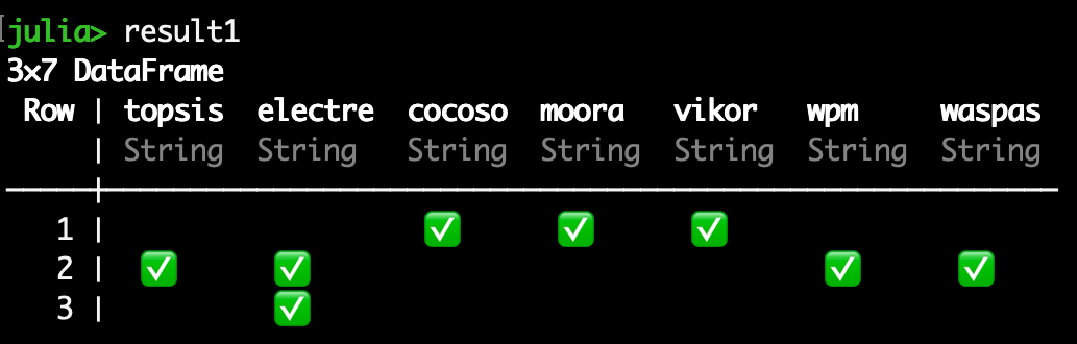
\includegraphics[width=\columnwidth]{images/result1}
	\caption{Results of TOPSIS, ELECTRE, VIKOR, MOORA, COCOSO, WPM, and WASPAS}
	\label{fig:imagea}
	\end{figure}

\begin{verbatim}
	julia> methods2 = [:aras, :saw, :edas, :marcos, 
	                   :mabac, :mairca, :grey];
	julia> result2 = summary(df, w, fns, methods2);
\end{verbatim}

Figure \ref{fig:imageb} represents the output of the \texttt{summary()} call for methods ARAS, SAW, EDAS, MARCOS, MABAC, MAIRCA, and GRA, respectively. Figure \ref{fig:imagea} and Figure \ref{fig:imageb} also show the necessity of using more than one decision-making tool as they produce different results for the same analysis.


	\begin{figure}
		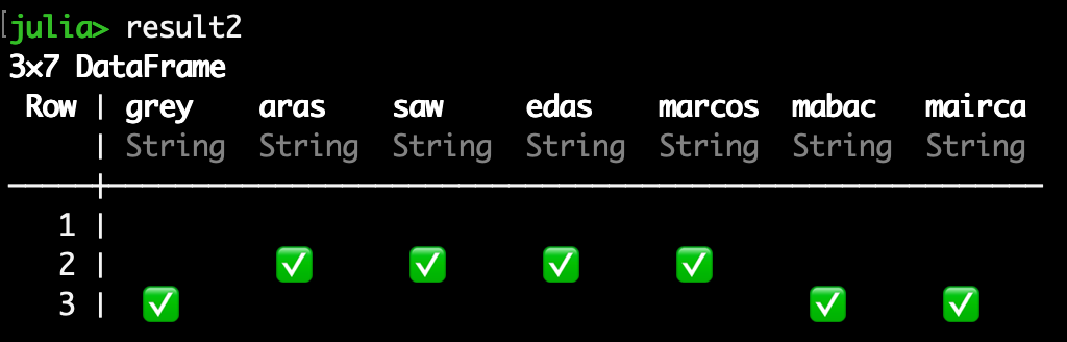
\includegraphics[width=\columnwidth]{images/result2}
		\caption{Results of ARAS, SAW, EDAS, MARCOS, MABAC, MAIRCA, and GRA}
		\label{fig:imageb}
		\end{figure}

%Optional: you may include one explanatory video that will appear next to your article, in the right hand side panel. (Please upload any video as a single supplementary file with your article. Only one MP4 formatted, with 50MB maximum size, video is possible per article. Recommended video dimensions are 640 x 480 at a maximum of 30 frames/second. Prior to submission please test and validate your .mp4 file at $ http://elsevier-apps.sciverse.com/GadgetVideoPodcastPlayerWeb/verification$. This tool will display your video exactly in the same way as it will appear on ScienceDirect.).

\section{Impact}
\label{section:impact}
%{\color{red}
%\textbf{This is the main section of the article and the reviewers weight the description here appropriately}
%Indicate in what way new research questions can be pursued as a result of the software (if any).
%Indicate in what way, and to what extent, the pursuit of existing research questions is improved (if so).
%Indicate in what way the software has changed the daily practice of its users (if so).
%Indicate how widespread the use of the software is within and outside the intended user group.
%Indicate in what way the software is used in commercial settings and/or how it led to the creation of spin-off companies (if so).
%}

\emph{JMcDM} provides a moderate number of MCDA tools and utility functions for developing new methods as well as performing
decision analysis using a single function call for each method. A researcher can easly perform sequantial analysis by changing 
the problem parameters and can compare results of many tools. Existing software packages are mainly focused on providing a 
small subset of methods. \emph{JMcDM} is an all-in-one solution and has potential for increasing user productivity. Seeing 
the different results produced by the methods together also helps to discover which parameters the research is more sensitive 
to and the reasons for them.   

\section{Conclusions}
\label{section:conclusion}
%{\color{red}Set out the conclusion of this original software publication.}
Multiple-criteria decision-making tools are used in various disciplines in the literature. Since it is difficult to compute these tools manually, many software packages and programs have been developed. However, these packages include a selected subset of methods. \emph{JMcDM} is a \emph{Julia} package that contains a significant amount of tools in the literature. Implementations of these tools are straightforward to use in \emph{Julia} REPL for researchers. \emph{JMcDM} also provides the necessary infrastructure for the development of new methods in the literature with its utility functions, comprehensive documentation, and unit tests compiled from many text books. The proposed package has also brought MCDA tools to a relatively new language such as \emph{Julia} with significant performance promises. The methods in the package are also designed to be familiar to users who previously used R and Python languages.

\section{Conflict of Interest}
%Please select the appropriate text:
%Potential conflict of interest exists:
%We wish to draw the attention of the Editor to the following facts, which may be considered as potential conflicts of interest, and to significant financial contributions to this work. The nature of potential conflict of interest is described below: [Describe conflict of interest]
%No conflict of interest exists:
We wish to confirm that there are no known conflicts of interest associated with this publication and there has been no significant financial support for this work that could have influenced its outcome.


\section*{Acknowledgements}
\label{section:Acknowledgements}

The authors would like to thankt he Editor-in-Chief, editors, reviewers for providing extremely insightful comments, and other stuff  of the SoftwareX Journal.

%% The Appendices part is started with the command \appendix;
%% appendix sections are then done as normal sections
%% \appendix

%% \section{}
%% \label{}

%% References:
%% If you have bibdatabase file and want bibtex to generate the
%% bibitems, please use
%%
\bibliographystyle{elsarticle-num} 
\bibliography{jmcdm}


%% else use the following coding to input the bibitems directly in the
%% TeX file.


%\begin{thebibliography}{00}
%% \bibitem{label}
%% Text of bibliographic item

%\bibitem{}

%\end{thebibliography}
%Please add the reference to the software repository if DOI for software  is available. 

%\section*{Current executable software version}
%\label{sec:current_executable_version}
%Ancillary data table required for sub version of the executable software: (x.1, x.2 etc.) kindly replace examples in right column with the correct information about your executables, and leave the left column as it is.

%\begin{table}[!h]
%\begin{tabular}{|l|p{6.5cm}|p{6.5cm}|}
%\hline
%\textbf{Nr.} & \textbf{(Executable) software metadata description} & \textbf{Please fill in this column} \\
%\hline
%S1 & Current software version & For example 1.1, 2.4 etc. \\
%\hline
%S2 & Permanent link to executables of this version  & For example: $https://github.com/combogenomics/$ $DuctApe/releases/tag/DuctApe-0.16.4$ \\
%\hline
%S3 & Legal Software License & List one of the approved licenses \\
%\hline
%S4 & Computing platforms/Operating Systems & For example Android, BSD, iOS, Linux, OS X, Microsoft Windows, Unix-like , IBM z/OS, distributed/web based etc. \\
%\hline
%S5 & Installation requirements \& dependencies & \\
%\hline
%S6 & If available, link to user manual - if formally published include a reference to the publication in the reference list & For example: $http://mozart.github.io/documentation/$ \\
%\hline
%S7 & Support email for questions & \\
%\hline
%\end{tabular}
%\caption{Software metadata (optional)}
%\label{software_metadata} 
%\end{table}

\end{document}
\endinput
%%
%% End of file `SoftwareX_article_template.tex'.
